%*******************************************************************************
%*******************************************************************************
\chapter{Songbook-Client}
\setcounter{chapter}{2}
\label{chap:songbook-client}
\minitoc
%*******************************************************************************
%*******************************************************************************

Le \client est interface graphique facilitant la création de
recueils de chansons personnalisés. Il s'agit d'un logiciel libre et
gratuit développé sur
\href{http://github.com/crep4ever/songbook-client}{Github}.

\begin{nota}
  Quel que soit votre système d'exploitation, il est nécessaire d'avoir
  installé au préalable les dépendances du \songbook lui-même
  (\refsec{sec:install}) afin de pouvoir produire un recueil PDF.
\end{nota}

Les téléchargements suivant les différents systèmes d'exploitation
sont proposés sur le site
\href{http://www.patacrep.com/fr/static1/downloads}{Patacrep!}


%*******************************************************************************
\section{Interface}
%*******************************************************************************

%-------------------------------------------------------------------------------
\subsection{Premier lancement}
%-------------------------------------------------------------------------------

\begin{figure}
  \centering
  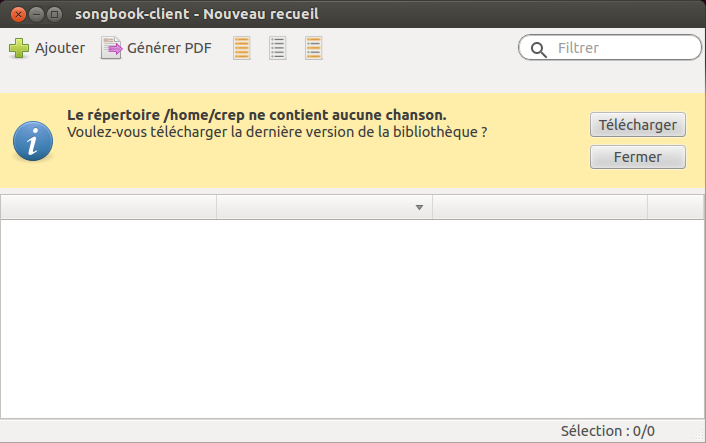
\includegraphics[width=\textwidth]{start}
  \caption{Premier lancement de l'application.}
  \label{fig:start}
\end{figure}

Par défaut, l'interface est vide (\reffig{fig:start}). Le
\client doit être lié à un \songbook existant. Vous avez
deux solutions~:

\begin{enumerate}
\item Vous pouvez indiquer le chemin d'un répertoire
  \directory{songbook} existant depuis le menu
  \menu{Édition}{Préférences} (\reffig{fig:solution-a}).
\item Vous pouvez télécharger la dernière version depuis internet
  depuis le menu \menu{Bibliothèque}{Télécharger}
  (\reffig{fig:solution-b}).
\end{enumerate}

Après avoir indiqué ou téléchargé un \songbook, le \client génère la
\emph{bibliothèque des chansons} trouvées dans le sous-répertoire
\directory{songs} du \songbook.


%%%%%%%%%%%%%%%%%%%%%%%%%%%%%% FIGURE %%%%%%%%%%%%%%%%%%%%%%%%%%%%%%%%%%
\begin{figure}
  \centering
  %% -- subfigures --
  \subfigure[]{
    \label{fig:solution-a}
    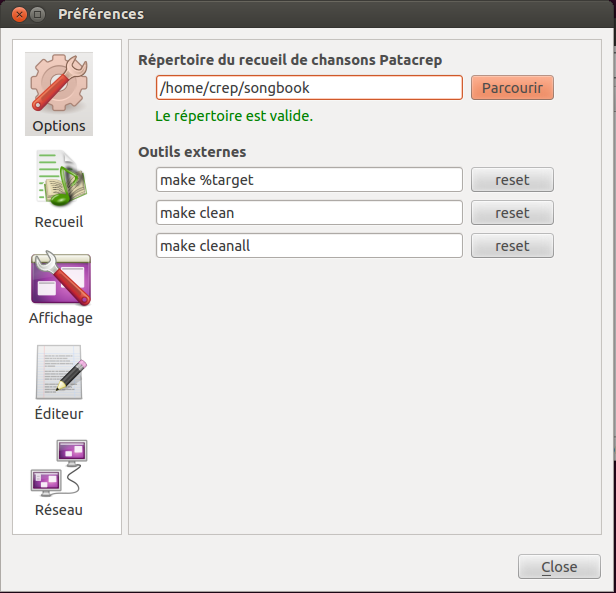
\includegraphics[width=0.45\textwidth]{preferences}%
  }%
  \hspace{0.1cm}%
  \subfigure[]{%
    \label{fig:solution-b}%
    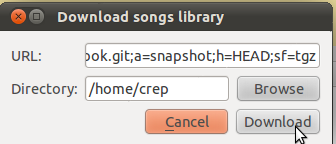
\includegraphics[width=0.45\textwidth]{download}%
  }%
  %% -- subfigures --
  \caption{% 
    Deux solutions permettent de lier le \emph{Songbook-Client} à un \songbook.
    \subref{fig:solution-a}~Indiquer le chemin d'un répertoire existant~;%
    \subref{fig:solution-b}~Télécharger depuis internet.%
  }%
  \label{fig:solutions}
\end{figure}
%%%%%%%%%%%%%%%%%%%%%%%%%%%%%%%%%%%%%%%%%%%%%%%%%%%%%%%%%%%%%%%%%%%%%%%%


%-------------------------------------------------------------------------------
\subsection{La bibliothèque des chansons}
%-------------------------------------------------------------------------------

\begin{figure}
  \centering
  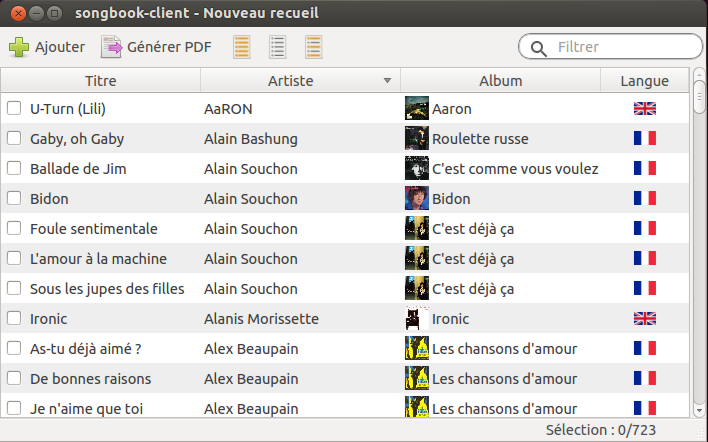
\includegraphics[width=\textwidth]{library}
  \caption{La bibliothèque des chansons.}
  \label{fig:library}
\end{figure}

L'ensemble des chansons \ext{sg} trouvées dans le sous-répertoire
\directory{songs} est présenté sous la forme d'une liste
(\reffig{fig:library}). Les différentes colonnes peuvent être
affichées/masquées dans l'onglet \command{Affichage} du menu
\menu{Édition}{Préférences}. Par défaut, seules les colonnes
\command{Titre}, \command{Artiste} et \command{Album} sont visibles.

Sélectionnez les chansons de la bibliothèque que vous souhaitez
inclure dans votre recueil avant de lancer la génération du PDF.

%-------------------------------------------------------------------------------
\subsection{L'éditeur de chansons}
%-------------------------------------------------------------------------------

\begin{figure}
  \centering
  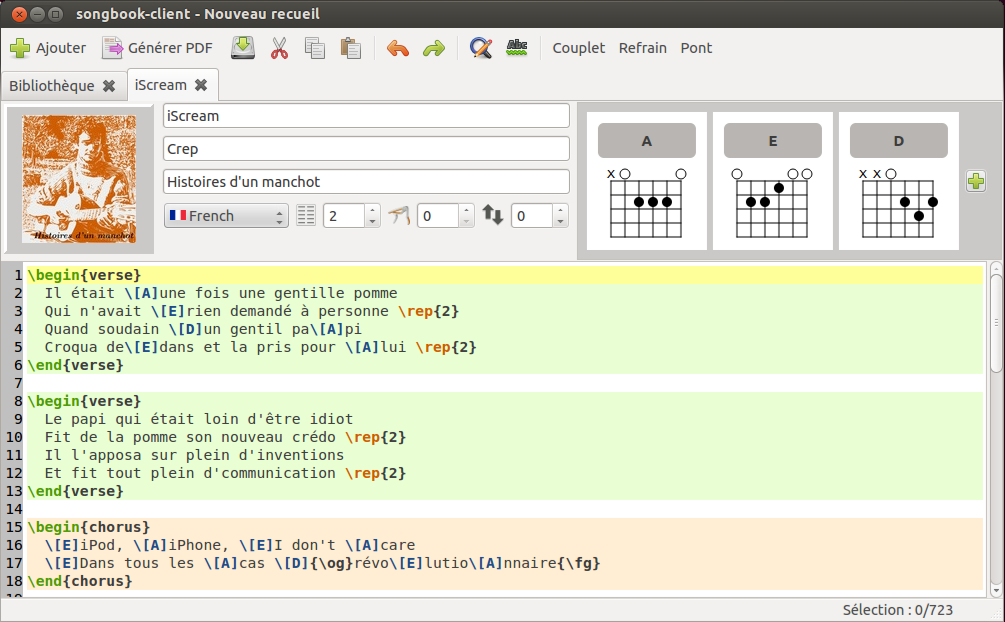
\includegraphics[width=\textwidth]{song-editor}
  \caption{L'éditeur de chansons.}
  \label{fig:song-editor}
\end{figure}

Les chansons présentes dans la bibliothèques peuvent être modifiées.
Pour cela, double-cliquez sur une chanson ou \menu{clic-droit}{Éditer}
pour ouvrir l'éditeur de chanson. L'éditeur est composé de deux
parties principales. Un ruban correspondant aux méta-données (titre,
artiste, album \dots) et un éditeur de texte pour le corps de la
chanson (\reffig{fig:song-editor}).

%-------------------------------------------------------------------------------
\subsection{Création d'un recueil personnalisé}
%-------------------------------------------------------------------------------

\paragraph{Enregistrement/Ouverture}
Le format de fichier \ext{sb} enregistre la liste des chansons
sélectionnées ainsi que son style et ses options
(voir~\refsec{sec:create-songbook}).

\paragraph{Style et options d'un recueil}
L'onglet \command{Recueil} du menu \menu{Édition}{Préférences} permet
de rapidement sélectionner le style du recueil pdf ainsi que les
différents éléments à faire apparaitre
(\reffig{fig:preferences-songbook}).

\begin{figure}
  \centering
  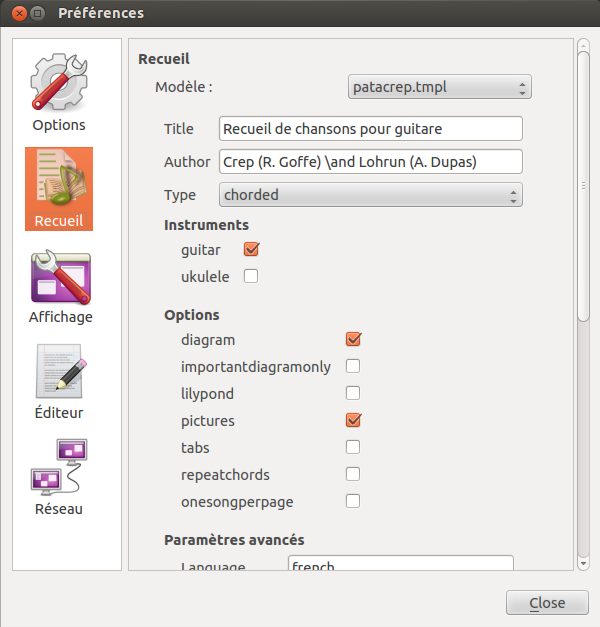
\includegraphics[width=.6\textwidth]{preferences-songbook}
  \caption{Personnalisation d'un recueil.}
  \label{fig:preferences-songbook}
\end{figure}

%*******************************************************************************
\section{Compilation depuis les sources}
%*******************************************************************************

Le \client est une application écrite en Qt/C++ dont la compilation
est gérée par \href{http://www.cmake.org}{CMake}.

%-------------------------------------------------------------------------------
\subsection{\linux}
%-------------------------------------------------------------------------------

\paragraph{Dépendances}

\begin{unix}
  sudo apt-get install build-essential cmake 
  sudo apt-get install qt4-qmake qt4-dev-tools
  sudo apt-get install libarchive-dev libhunspell-dev
\end{unix}

Les dépendances à
\href{http://code.google.com/p/libarchive/}{libarchive} et
\href{http://hunspell.sourceforge.net/}{libhunspell} sont facultatives
à la compilation du \client mais les fonctionnalités comme le
téléchargement de la bibliothèque et la correction orthographique en
dépendent.

\paragraph{Téléchargement}

\begin{unix}
  git clone git://github.com/crep4ever/songbook-client.git
\end{unix}

\paragraph{Compilation/Exécution}

\begin{unix}
  cd songbook-client
  make && sudo make install
  songbook-client
\end{unix}

%-------------------------------------------------------------------------------
\subsection{\windows}
%-------------------------------------------------------------------------------

Téléchargez et installez la dernière version du
\href{http://qt.nokia.com/downloads}{SDK Qt}. Lancez QtCreator puis
choisissez \menu{Fichier}{Ouvrir un nouveau fichier} et sélectionnez
le fichier \file{CMakeList.txt} situé à la racine du répertoire des
sources du \client (\reffig{fig:qtcreator-a}). Cliquez sur
\Key{Éxécuter CMake} (\reffig{fig:qtcreator-b}). Votre projet \client
est maintenant configuré, lancez la compilation avec
\Key{Ctrl}+\Key{r} (\reffig{fig:qtcreator-c}).

%%%%%%%%%%%%%%%%%%%%%%%%%%%%%% FIGURE %%%%%%%%%%%%%%%%%%%%%%%%%%%%%%%%%%
\begin{figure}
  \centering
  %% -- subfigures --
  \subfigure[]{
    \label{fig:qtcreator-a}
    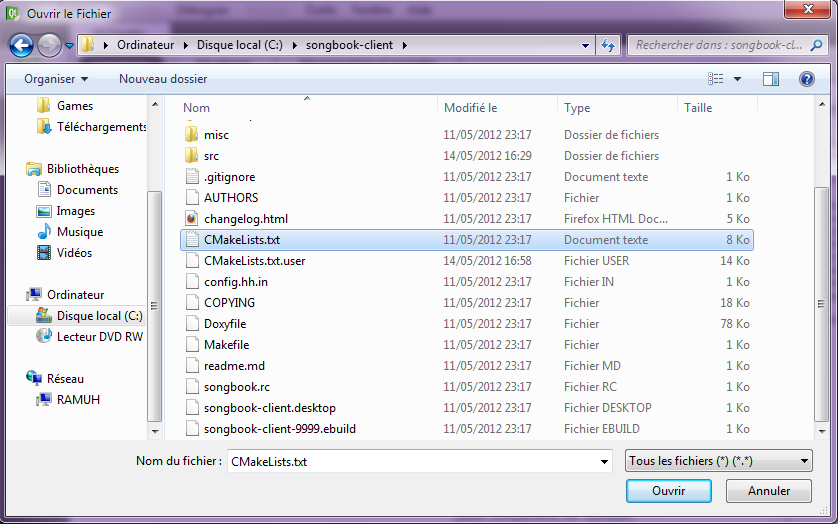
\includegraphics[width=0.6\textwidth]{qtcreator-a}%
  }%
  \hspace{0.1cm}%
  \subfigure[]{%
    \label{fig:qtcreator-b}%
    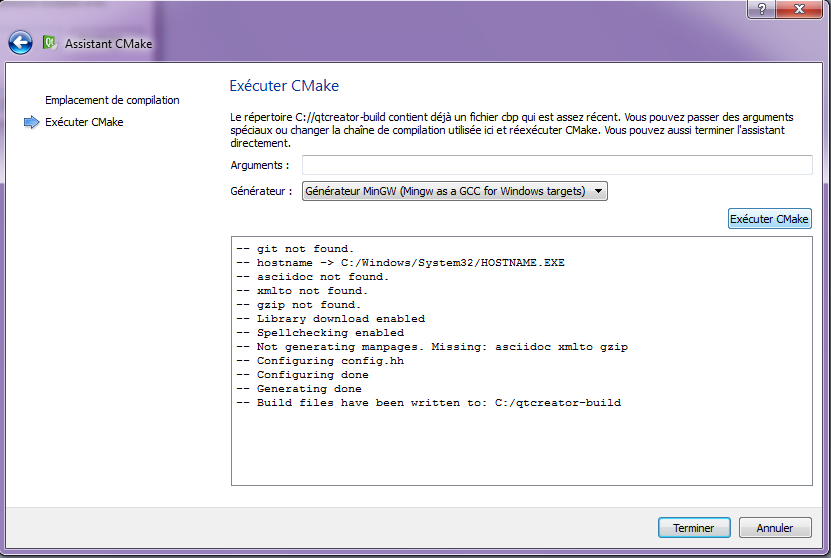
\includegraphics[width=0.6\textwidth]{qtcreator-b}%
  }%
  \hspace{0.1cm}%
  \subfigure[]{%
    \label{fig:qtcreator-c}%
    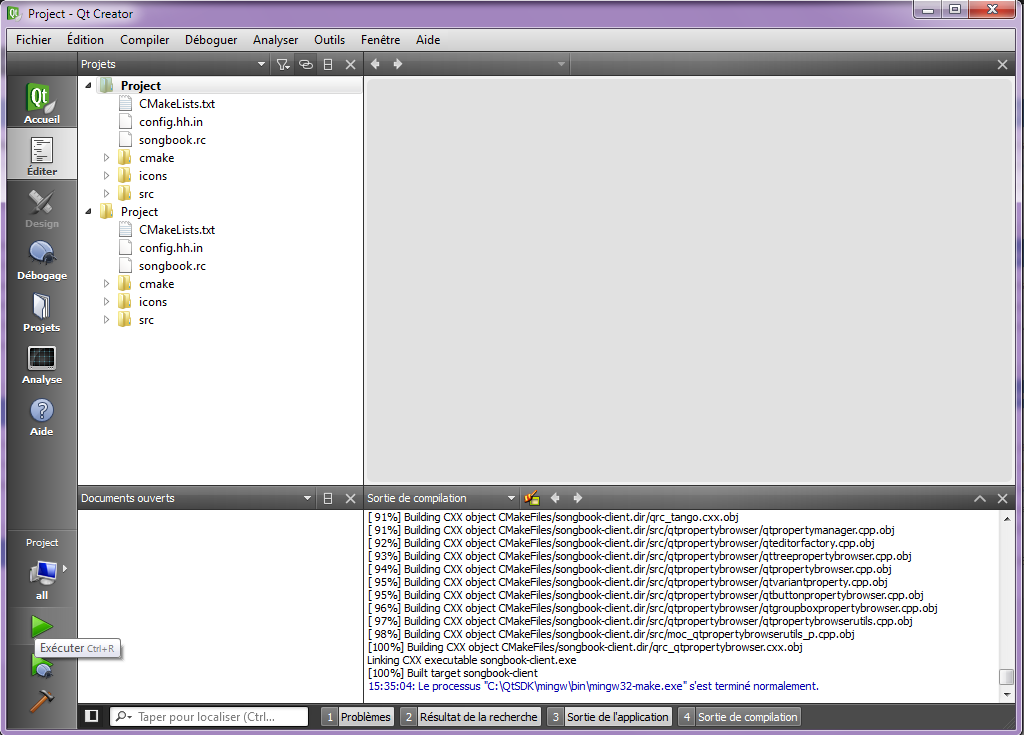
\includegraphics[width=0.6\textwidth]{qtcreator-c}%
  }%
  %% -- subfigures --
  \caption{% 
    Compilation des sources du \songbook avec QtCreator.
    \subref{fig:qtcreator-a}~Ouverture du projet~;%
    \subref{fig:qtcreator-b}~Configuration avec CMake~;%
    \subref{fig:qtcreator-c}~Compilation.%
  }%
  \label{fig:qtcreator}
\end{figure}
%%%%%%%%%%%%%%%%%%%%%%%%%%%%%%%%%%%%%%%%%%%%%%%%%%%%%%%%%%%%%%%%%%%%%%%%

%TODO: libarchive et libhunspell

%*******************************************************************************
\section{FAQ}
%*******************************************************************************

\paragraph{Comment signaler un bug ?}
Directement sur \href{http://github.com/crep4ever/songbook-client/issues}{Github}
ou via le \href{http://www.patacrep.com/forum/}{forum Patacrep!}

\paragraph{Les partitions Lilypond n'apparaissent pas}
Si la compilation de votre recueil de chansons n'intègre pas les
partitions malgré l'option \emph{Lilypond} correctement cochée dans
les préférences, vérifiez que Lilypond est bien installé sur votre
système. Sous MacOs et Windows, il est nécessaire de générer soi-même
les pdf correspondants aux partitions, le processus n'étant pas
automatisé par le makefile.

\paragraph{La bibliothèque des chansons est vide} 
Vérifiez que le chemin d'accès au \songbook est correctement
renseigné dans \menu{Édition}{Préférences}. Le chemin indiqué doit contenir
impérativement le makefile et le répertoire \directory{songs/}.

\paragraph{Erreurs après renommage/suppression d'une chanson} 
Un \command{make clean} ou, depuis l'interface, \menu{Recueil}{Nettoyer} devrait
régler le problème. S'il persiste encore, une solution radicale
consiste à supprimer manuellement tous les fichiers \ext{d} présents
dans \directory{$\sim$/songbook}.
